%%\section{Notion [E]}
%%\setauthor{Ema Halilovic}
%%Notion ist eine Software, mit der so genannte \emph%%{Workspaces} erstellt werden können. 
%%Diese ist verfügbar im Browser, als App in Windows-, MacOS- %%oder auf iOS- und Android-Geräten. 
%%Es besteht die Möglichkeit eine Seite zu erstellen und mit %%einem einzigen Befehl Unterseiten anzulegen, welche direkt %%verlinkt werden.
%%Diese Seiten lassen sich mit beliebigem Inhalt füllen und %%durch einfache ""/""-Befehle ist es möglich z. B. ein Kanban %%Board erstellen. 
%%Es ist sehr einsteigerfreundlich, da alle Funktionalitäten gut %%beschrieben sind und es benutzerfreundlich gestaltet ist.
%%Workspaces lassen sich mit anderen Nutzern teilen, wodurch %%jeder Nutzer auf eine \emph{single soruce of truth} Version %%des Workspaces zugreifen kann.
%%Für die Bearbeitung in echt-Zeit wird Internet benötigt, falls %%dieses jedoch ausfällt, werden die Änderungen gespeichert und %%synchronisiert, sobald wieder eine Netzwerkverbindung %%aufgebaut wurde.
%%\cite{NotionAbout}
%%
%%Das Feature von geteilten Workspaces war für diese Arbeit %%nützlich, um Notizen nach Meetings und gemeinsame Termine %%festzuhalten, genauso um wichtige Links zu speichern und diese %%schnell wieder abrufen zu können.
%%
%%\begin{figure} [h t]
%%  \centering
%%  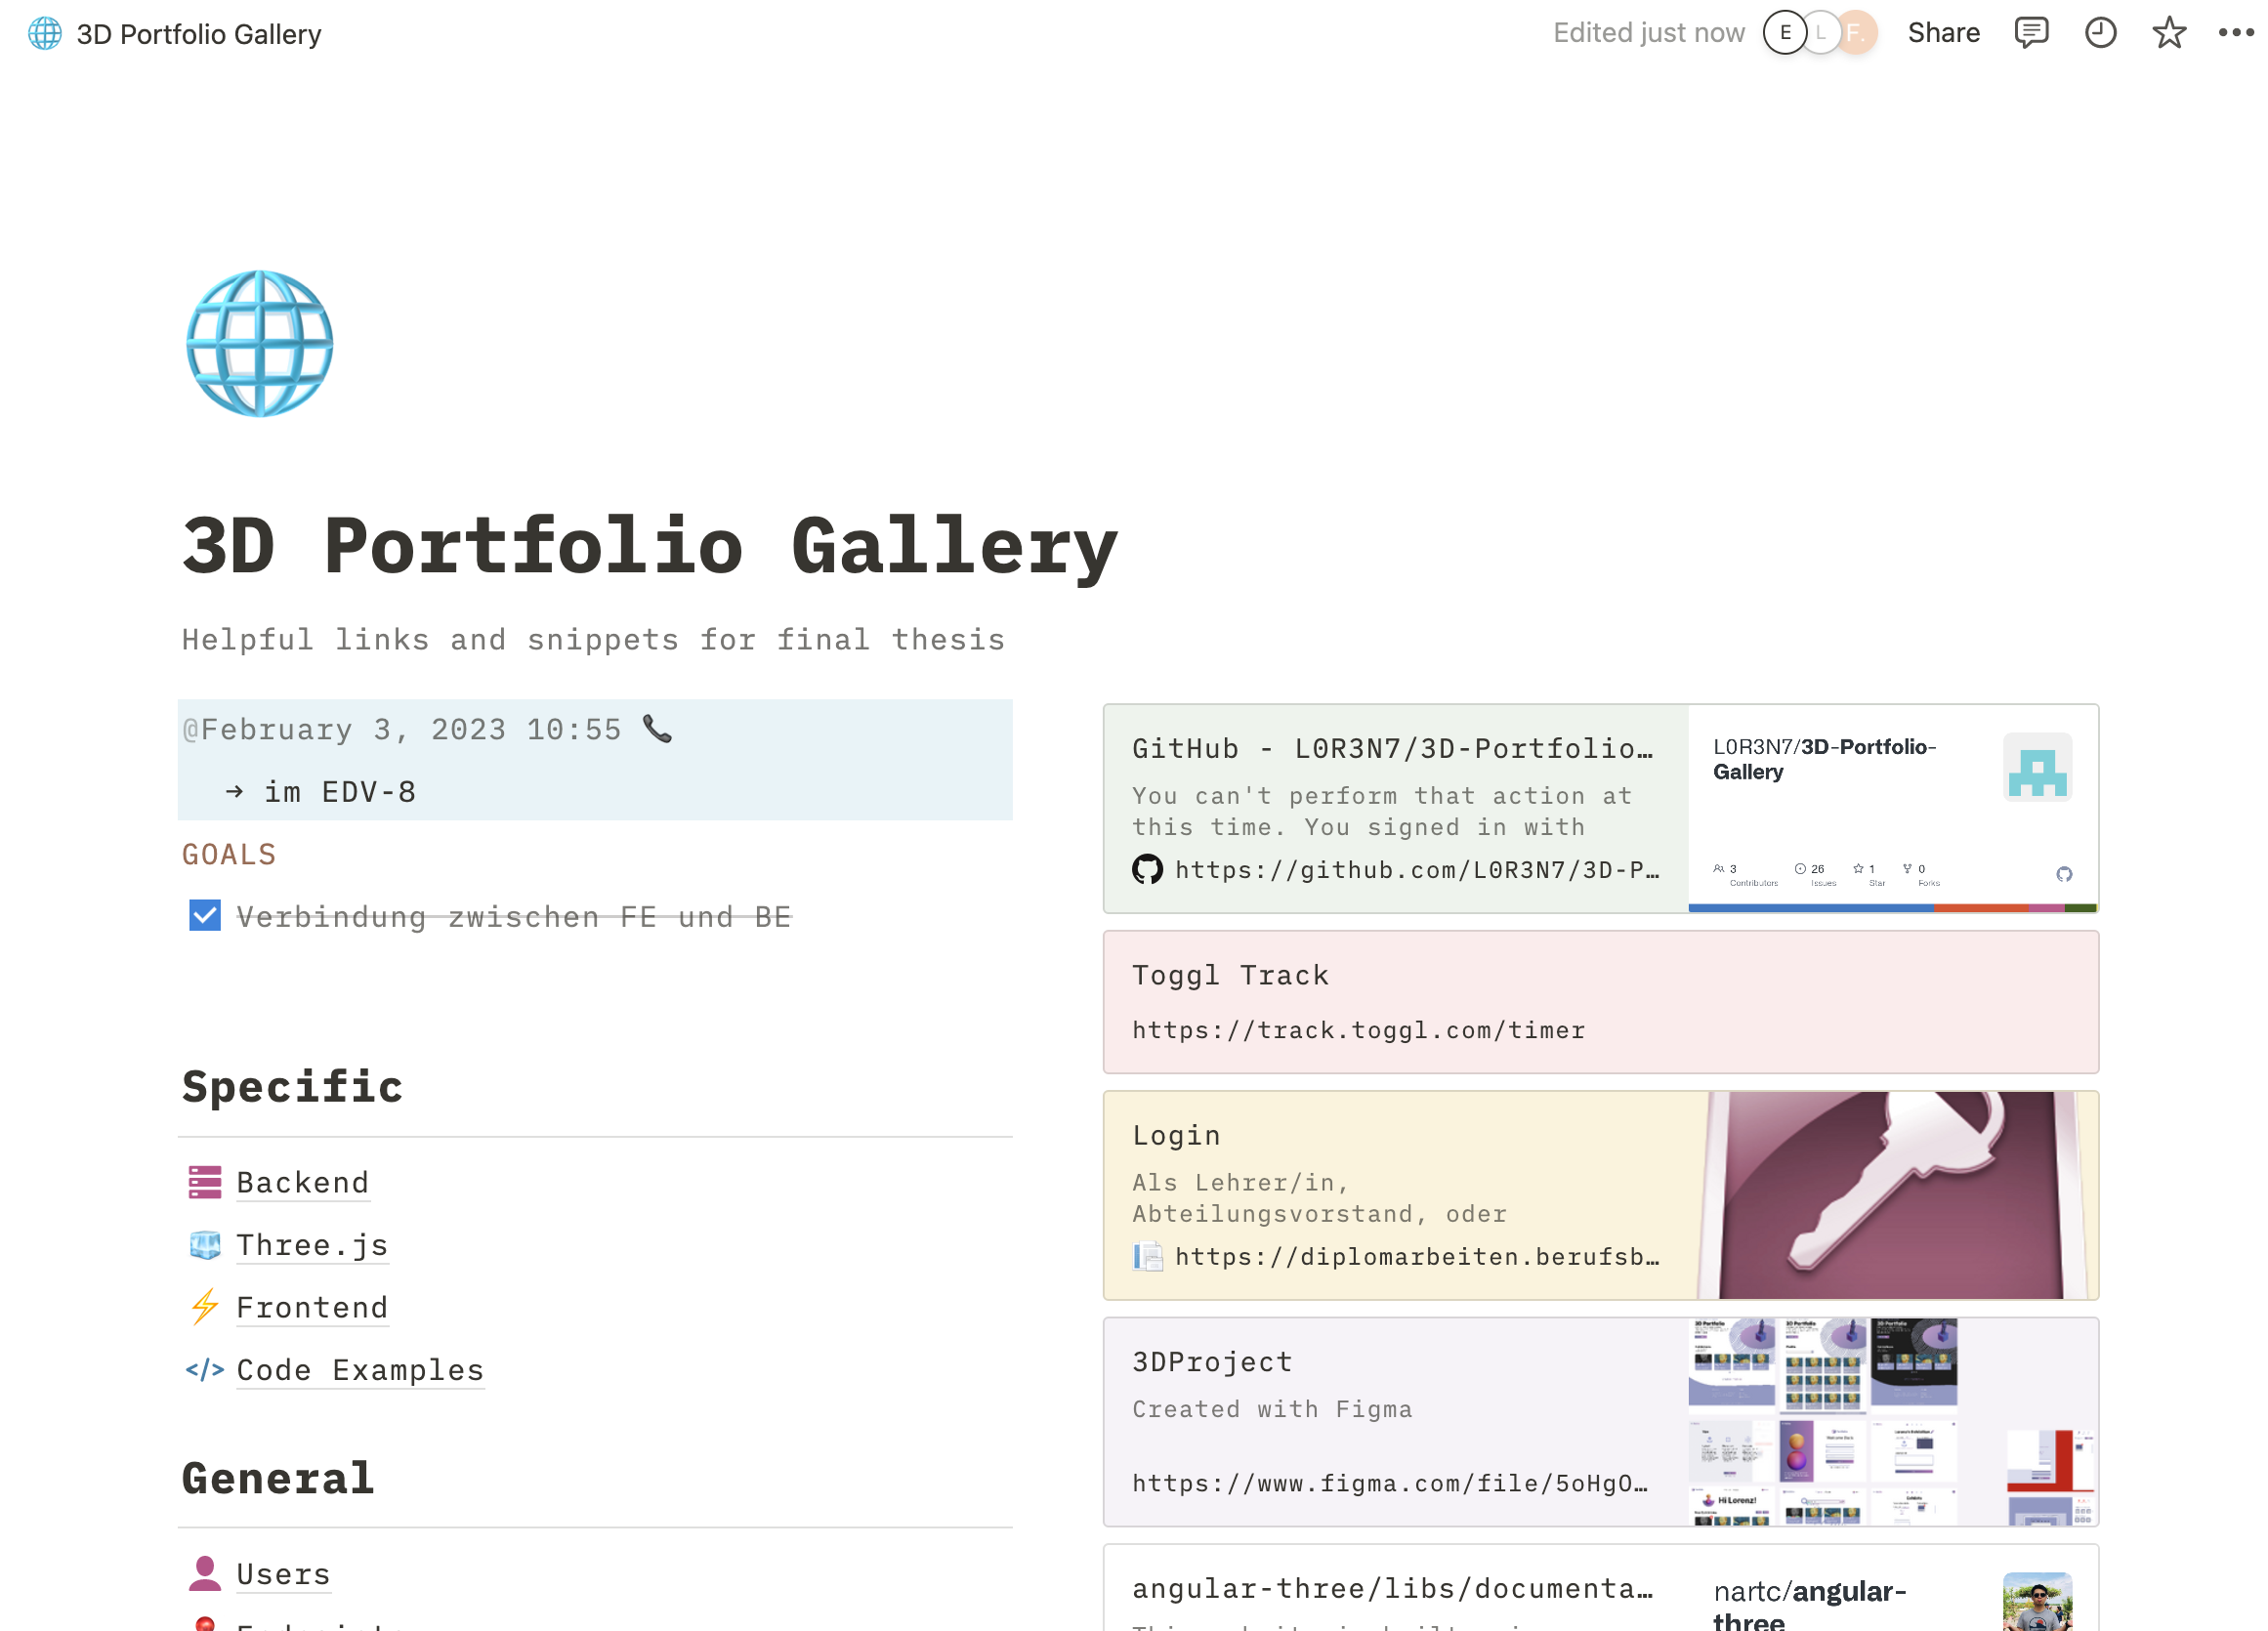
\includegraphics[scale=0.3]{pics/NotionPage.png}
%%  \caption{Notion Workspace der Diplomarbeit}
%%  \label{fig:tech:notion-page}
%%\end{figure}
%%
%%\section{PlantUML [E]}
%%\setauthor{Ema Halilovic}
